\chapter{Related work}

\section{Image forgery}

When dealing with a digital image, it is quite common to wonder if it is original or has been counterfeited in some way. Images and videos have become the main information carriers in the digital era and used to store real world events, but  they are very easy to manipulate because of the availability of the powerful editing software and sophisticated digital cameras.

The contexts where doctored pictures could be involved are very disparate; they could be used in a tabloid or in an advertising poster or included in a journalistic report but also in a court of law where digital (sometimes printed) images are presented as crucial evidences for a trial in order to influence the final judgement. So, especially in the last case, reliably assessing image integrity becomes of fundamental importance. 

\emph{Image forensics} specifically deals with such issues by studying and developing technological tools which generally permit determining, by only analyzing a digital photograph (i.e., its pixels), if that asset has been manipulated or even which could have been the adopted acquisition device (such an issue is not relevant to the topic of the present paper). Moreover, if it has been established that something has been altered, it could be important to understand in which part of the image itself such a modification occurred, for instance, if a person or a specific object has been covered, if an area of the image has been cloned, if something (i.e., a face or a weapon) has been copied from another different image, or, even more, if a mixture of these processes has been carried out. 

\section{Image forgery detection techniques}

To verify the authenticity of a picture many techniques have been identified that can be categorized into active (intrusive) and blind (non-intrusive).

Operative techniques involve a phase of preprocessing the image itself at the time of its creation in order to include some additional information that will be used during the analysis phase. An example of operative technique is the watermarking.

Passive techniques analyze the content of the image using various statistics or semantic content in order to identify inconsistencies of some kind. This approach does not alter the contents of the image.
There is a general technique, suitable to capture all kinds of inconsistencies present in an image, but each different method specialises in the identification of a particular type.

\section{Image splicing}

Image splicing is a very common type of infringement which basically consists in copying a region of a given image to another, thus creating a composition of two different pictures together.

\begin{figure}
  \centering
    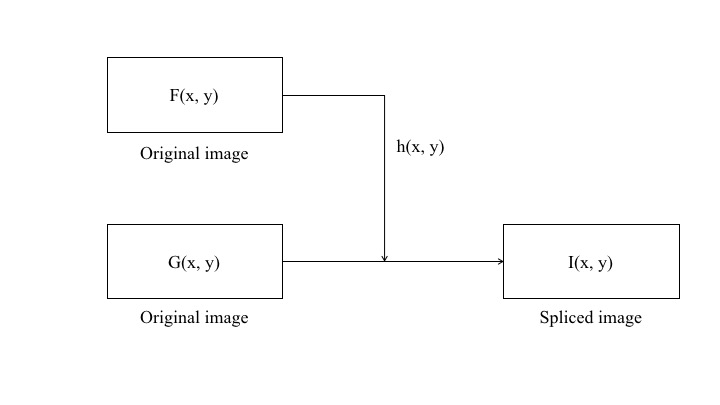
\includegraphics[width=0.8\textwidth]{imagesplicing}
    \caption{Image splicing process}
\end{figure}


\subsection{Some famous cases}

Photography has lost its innocence since the early days of his birth. In fact already in 1860, only a few decades after Niépce created the first photo, the first manipulated photographs were identified in 1826. With the advent of digital cameras, camcorders and sophisticated photo editing software, digital image manipulation is becoming more common. 

\paragraph{O.J. Simpson - June 1994}

This altered photography O.J. Simpson appeared on the cover of the magazine Time Magazine, soon after his arrest for murder. 

\begin{wrapfigure}{r}{0.5\textwidth}
  \begin{center}
    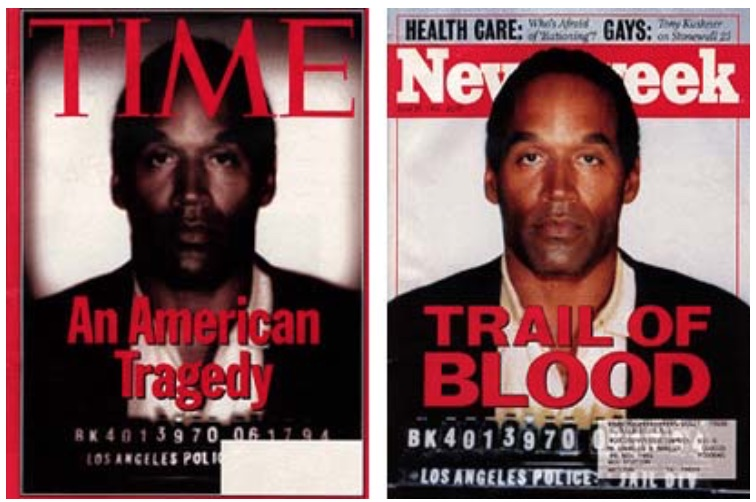
\includegraphics[width=0.48\textwidth]{ojsimpson}
  \end{center}
  \caption{The Time Magazine and O.J. Simpson}
  \vspace{-1cm}
\end{wrapfigure}

In fact, the photograph was altered compared to the original image that has appeared on the cover of Newsweek magazine. Time magazine was accused of manipulation of the photography in order to make darker and menacing figure of Simpson.

\paragraph{Iraq - April 2003}

This composition of a British soldier in Basra, which keeps pointing toward a civilian Iraqi gesticulates covered, she appeared on the cover of the Los Angeles Times, immediately after the invasion of Iraq. 

\begin{wrapfigure}{l}{0.5\textwidth}
  \begin{center}
    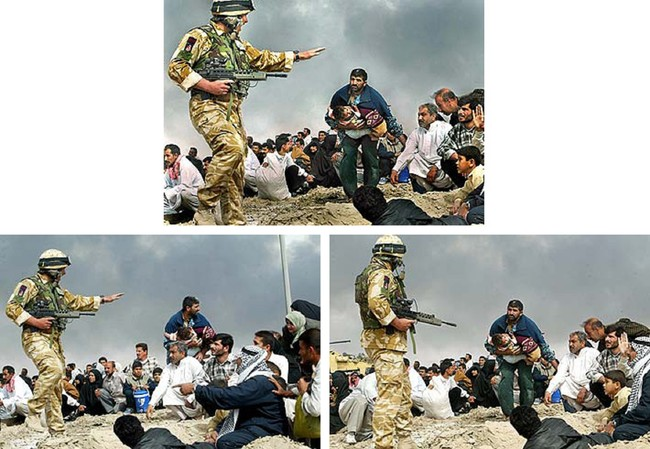
\includegraphics[width=0.48\textwidth]{iraq}
  \end{center}
  \caption{An example of image composition}
\end{wrapfigure}

Brian Walski, a staff photographer for the Los Angeles Times and a veteran of the news with thirty years of experience, was summarily fired from his publisher for their merged two of his shots in order to improve the composition.

\paragraph{George W. Bush - March 2004}

This image, taken from promo released for the election campaign of George w. Bush, outlined a packed audience of soldiers as a backdrop to a child who was flying the American flag. This image was digitally souped-up, using a crude copy and paste, removing Bush from the podium. 

\begin{wrapfigure}{r}{0.5\textwidth}
  \begin{center}
    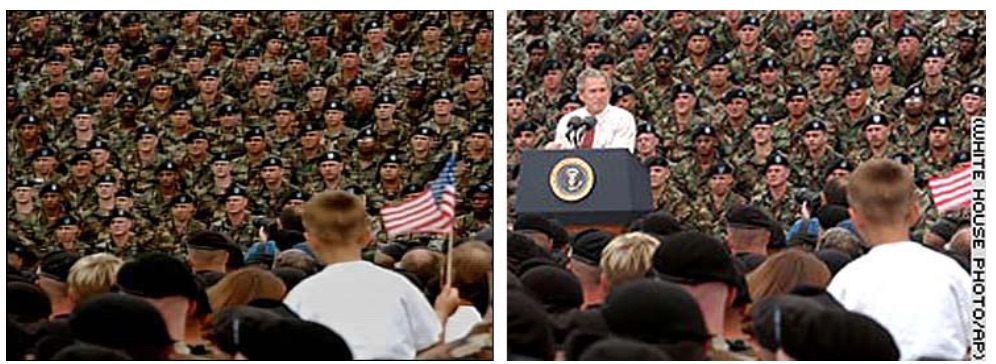
\includegraphics[width=0.48\textwidth]{bush}
  \end{center}
  \caption{An example of image composition}
\end{wrapfigure}


After admitting the tampering with the staff of the television station edited and sent to Bush promo with the original photo.

\section{Methods based on light inconsistencies}